%!TEX TS-program=xelatex
%!USE flag=shell-escape
\documentclass{beamer}
\usepackage{HSE-theme/beamerthemeHSE} % Подгружаем тему

%%% Работа с русским языком и шрифтами
\usepackage[english,russian]{babel}   % загружает пакет многоязыковой вёрстки
\usepackage{fontspec}      % подготавливает загрузку шрифтов Open Type, True Type и др.
\defaultfontfeatures{Ligatures={TeX},Renderer=Basic}  % свойства шрифтов по умолчанию
\setmainfont[Ligatures={TeX,Historic}]{Myriad Pro} %  установите шрифты Myriad Pro или (при невозможности) замените здесь на другой шрифт, который есть в системе — например, Arial
\setsansfont{Myriad Pro}  %  установите шрифты Myriad Pro или (при невозможности) замените здесь на другой шрифт, который есть в системе — например, Arial
\setmonofont{Courier New}
\uselanguage{russian}
\languagepath{russian}
\deftranslation[to=russian]{Theorem}{Теорема}
\deftranslation[to=russian]{Definition}{Определение}
\deftranslation[to=russian]{Definitions}{Определения}
\deftranslation[to=russian]{Corollary}{Следствие}
\deftranslation[to=russian]{Fact}{Факт}
\deftranslation[to=russian]{Example}{Пример}
\deftranslation[to=russian]{Examples}{Примеры}

\usepackage{multicol} 		% Несколько колонок
\graphicspath{{images/}}  	% Папка с картинками

%%% Информация об авторе и выступлении
\title[Заголовок]{\footnotesize Факультет Компьютерных Наук\\Департамент
Программной Инженерии\\Курсовая работа}
\subtitle{Клиент-Серверное Приложение для Управления Скидками в Розничных Сетях}
\author[Куприянов К.И.,\smallskip Суровцев М.А.]{\scriptsize Выполнили студенты
гр.БПИ151\\Куприянов Кирилл\\Суровцев Максим\\Научный руководитель:\\Профессор
ДПИ Александров Дмитрий Владимирович}
\institute[Высшая школа экономики]{}
\date{\the\year}

\begin{document}	% Начало презентации
\frame[plain]{
    \maketitle
}

% \frame[plain]{\titlepage}	% Титульный слайд

% \section{Просто слайд с текстом}
% \subsection{Просто слайд с текстом}

\begin{frame}
\frametitle{Предметная область}
	\begin{multicols}{2}
        Агрегаторы скидок - место, где собрана вся информация об акционных товарах и выгодных предложениях.
		\columnbreak
		\medskip
		
\includegraphics[width=\columnwidth]{skidka.png}
	\end{multicols}
\end{frame}

\begin{frame}
\frametitle{Основные определения}
	\begin{enumerate}
		\item Crawler --- Программный модуль, работающий в фоне и производящий
            сбор данных с сайтов указанных магазинов, с последующей отправкой
            их на сервер в формате JSON
		\item REST API --- Стиль архитектуры программного обеспечения для построения веб-сервисов с использованием протокола HTTP.
    \item ORM --- технология программирования, которая связывает базы
      данных с концепциями объектно-ориентированных языков программирования,
      создавая «виртуальную объектную базу данных».
    \item Activity --- компонент приложения, с
      которым пользователи могут взаимодействовать для выполнения
      каких-либо действий
	\end{enumerate}
\end{frame}

\begin{frame}[c]
    \frametitle{Обоснование актуальности работы}
    \framesubtitle{Популярность скидок в интернете}
    \begin{figure}
        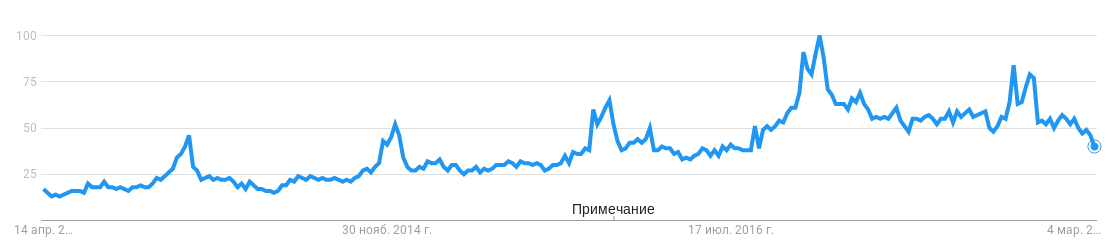
\includegraphics[width=\columnwidth]{trend.png}
        \caption{Статистика запроса ``скидки'' в Google}
    \end{figure}
    \begin{figure}
        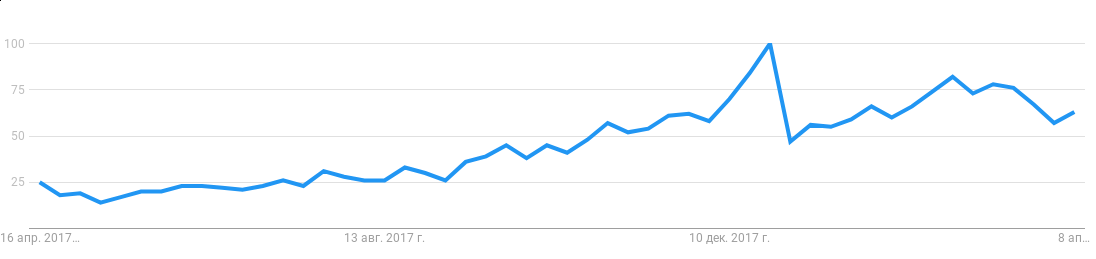
\includegraphics[width=\columnwidth]{trend_edadeal.png}
        \caption{Статистика запроса ``Едадил'' в Google}
    \end{figure}
\end{frame}

\begin{frame}
    \frametitle{Обоснование актуальности работы}
    \framesubtitle{Проблема}
    \begin{enumerate}
        \item Рост количества страниц со скидками на отдельных сайтах магазинов
        \item Разный дизайн и архитектура сайтов магазинов
        \item Отсутствие приложений с функционалом создания нескольких списков покупок
            % Люди стремятся экономить, но разный дизайн сайтов магазинов и отсутствие у некоторых магазинов сайтов впринципе, усложняет их задачу.
    \end{enumerate}
\end{frame}

\begin{frame}
    \frametitle{Цель и задачи работы}
    Цель работы --- реализовать модульные и масштабируемые web и Android
    приложения для работы со множеством скисков покупок, просмотра и управления
    акциями в розничных сетях\\
    \bigskip
    Задачи работы
    \begin{enumerate}
        \item Изучить существующие аналоги данного приложения
        \item Выбрать технологии для реализации
        \item Продумать модульность архитектуры
        \item Реализовать программу
        \item Разработать техническую документацию
            % Люди стремятся экономить, но разный дизайн сайтов магазинов и отсутствие у некоторых магазинов сайтов впринципе, усложняет их задачу.
    \end{enumerate}
\end{frame}

\begin{frame}
\frametitle{Анализ существующих решений}
    Едадил — акции в магазинах (бета)
        \medskip
        \begin{center}
        
\includegraphics[width=0.5\columnwidth]{edadeal.png}
        \end{center}
\end{frame}

\begin{frame}
    % -------------------------------
    % Особенности нашего приложения, которые выделяют нас не только среди аналогов, но и как программный продукт.
    % -------------------------------
    % -------------------------------
    % -------------------------------
\frametitle{Преимущества перед аналогами}
	\begin{multicols}{2}
        Удобство использования
        \bigskip
        \begin{itemize}
            \item Неограниченное количество списков покупок
            \item В список можно даже добавить товар, которого нет в магазине
            \item Использование одного аккаунта несколькими людьми
        \end{itemize}
	\columnbreak
        Архитектура
        \bigskip
	\begin{itemize}
		\item Модульность
		\item Масштабируемость
		\item Поддерживаемость
	\end{itemize}
	\end{multicols}
\end{frame}

\begin{frame}
    \frametitle{Алгоритм работы программы}
    \framesubtitle{Crawler}
    \begin{multicols}{2}
        \begin{itemize}
            \item Собирает данные с сайтов
            \item Селекторы: xpath
            \item Разбит на модули
                \begin{itemize}
                    \item spiders (1 паук на магазин)
                    \item selectors (1 селектор на магазин)
                    \item text\_processors
                    \item pipelines
                \end{itemize}
        \end{itemize}
        \bigskip
        \columnbreak
        \begin{figure}
            
\includegraphics[width=0.8\columnwidth]{crawler.png}
        \end{figure}
    \end{multicols}
\end{frame}


\begin{frame}[fragile]
    \frametitle{REST API}

    /api/shops/\textcolor{red}{1}\textcolor{cyan}{?category=Напитки\&page=1}
    \medskip
    \begin{minted}{json}
    {
      "count": 9,
      "numPages": 1,
      "rows": [
        {
          "id": 142138,
          "name": "Холодный чай Nestea вкус лимона, 0,5 л",
          "category": "Напитки",
          "oldPrice": 66.2,
          "newPrice": 44.99,
          "dateIn": "2018-04-09",
          "dateOut": "2018-04-15",
          "crawlDate": "2018-04-11",
          "condition": "-",
          "image": null,
          "imageUrl": "https://dixy.ru/upload/iblock/ea9/2000003636.jpg",
          "discount": "-32",
          "shop": {
              "id": 1,
              "alias": "dixy",
              "name": "Дикси"
          }
        }
      ]
    }
    \end{minted}
\end{frame}

\begin{frame}
    \frametitle{База данных}
    \medskip
    \begin{center}
      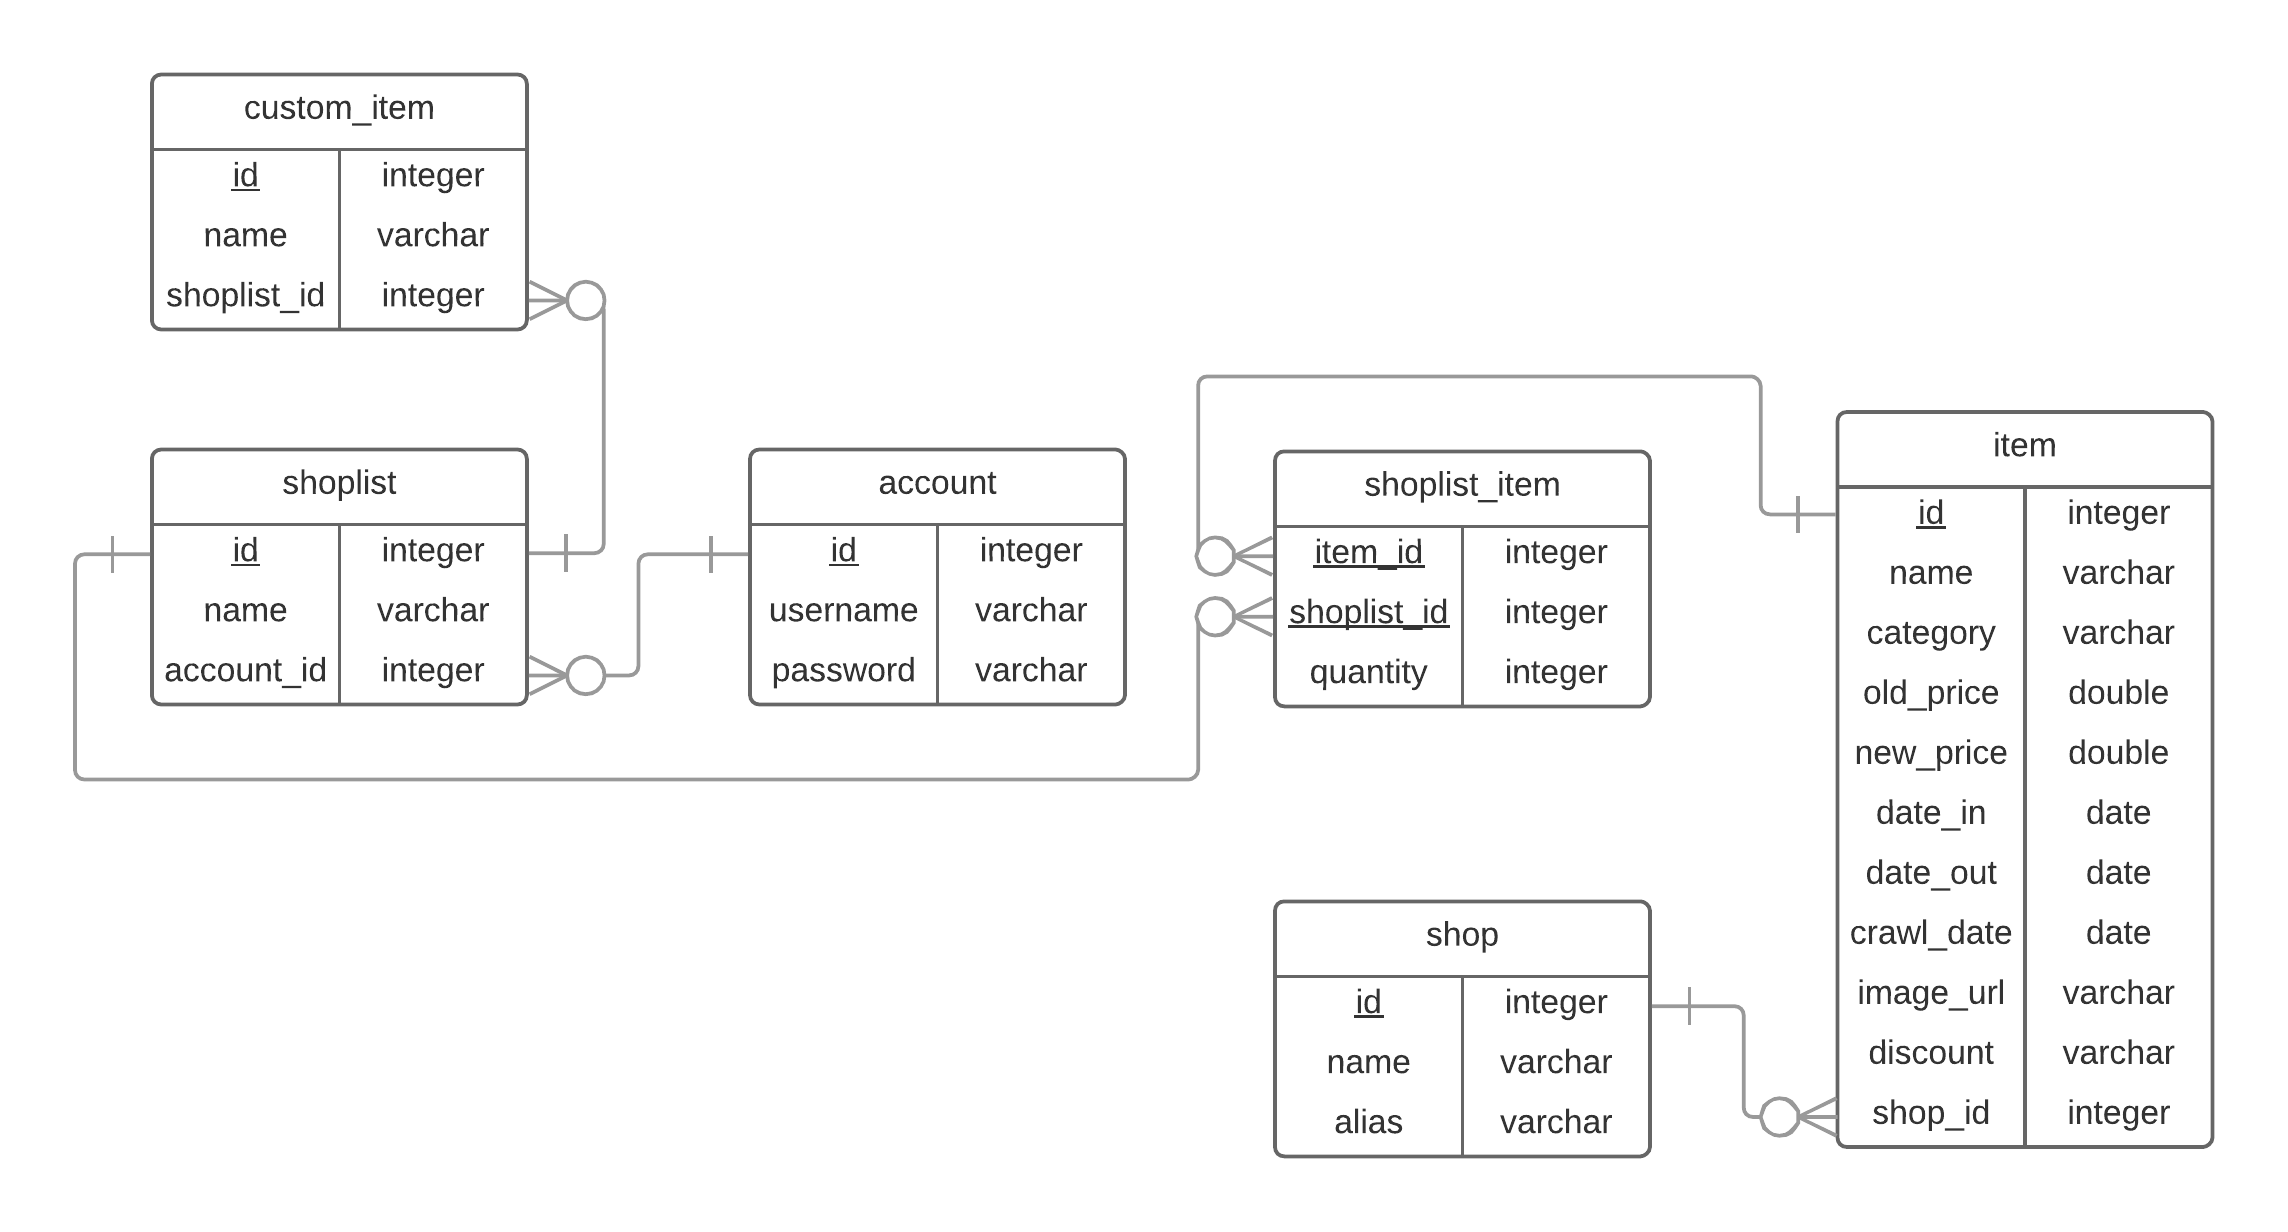
\includegraphics[width=\linewidth]{database}
    \end{center}
\end{frame}

\begin{frame}
    \frametitle{Результаты работы}
    asdf
\end{frame}

\begin{frame}
    \frametitle{Выводы по работе}
    asdf
\end{frame}

\begin{frame}
    \frametitle{Список используемых источников}
    asdf
\end{frame}

\begin{frame}[c]
\begin{center}
\frametitle{\LARGE Спасибо за внимание!}

{\LARGE \inserttitle}

\bigskip

{\insertauthor}

\bigskip\bigskip

{\insertinstitute}

\bigskip\bigskip

{\large \insertdate}
\end{center}
\end{frame}

\begin{frame}[c]
\begin{center}
\frametitle{\LARGE Ссылки на приложение}

    \url{www.4pda.ru/forum/index.php?showtopic=897451}
    \bigskip\\
    \bigskip\bigskip
    \url{www.gcsales.ru}

\end{center}
\end{frame}

\end{document}


% EOF

